\documentclass[12pt]{beamer}
\usetheme{UMNGolphers}

\usepackage[utf8]{inputenc}
\usepackage[T1]{fontenc}
\usepackage{helvet}
\usepackage{color}
\usepackage{topcapt}
\usepackage[english]{babel}
\usepackage{feynmf}
\usepackage{feyn}




\title{\LARGE SUSY Models: Non-Prompt Decays}
%\vskip400pt
%\subtitle{ UMN Delayed Photon Meeting}
\author{Tambe E. Norbert}
\date{\today}
%\institute{\url{norbert@physics.umn.edu}\\\url{http://www.physics.umn.edu/people/norbert.html}}
\institute{ University of Minnesota, \\ Email: \url{norbert@physics.umn.edu}}


\begin{document}
% Align Titile in center
\begin{frame}[c]
\titlepage
\end{frame}
\section{Outline}
\begin{frame}
\frametitle{Outline}
\tableofcontents
\end{frame}

\section{Introduction}
\begin{frame}
\frametitle{Introduction}
%\framesubtitle{Bullet points}
\begin{enumerate}


\item Non-prompt decay of SUSY particles  occur in the following SUSY breaking models:
	\begin{itemize}
	\item  Minimal Gauge Mediating SUSY Breaking (\textbf{GMSB})
	\item General Gauge Mediating SUSY Breaking (\textbf{GGM})
	\item Pure General Gauge Mediating SUSY Breaking (\textbf{PGGM})
	\end{itemize}
\item  These models predict the existence of a Next-to-lightest sparticle~(NLSP) decaying to a lightest sparticle~(LSP).
\item The LSP can be (non)stable depending on  R-Parity conserving(violation)~RPC(RPV). 
\item In RPC, NLSP decays to Gravitino($\tilde{G}$)) and SM-partner($\gamma,Z(\ell^{+}\ell^{-}),\mbox{Higgs}$).
\item Focus: Scenario where NLSP could be any SUSY particle decaying to a \alert{photon} i.e $\tilde{NLSP}\rightarrow \gamma + \tilde{G}$
\end{enumerate}
\end{frame}

\section{SUSY Models}
\begin{frame}
\frametitle{NLSP SUSY Models}
SUSY models are defined by a set of parameters.
\begin{enumerate}
\item GMSB
\begin{itemize}
 \item $\displaystyle{\Lambda = \frac{\left\langle F_{S}\right\rangle}{M_{\mbox{m}}}:\mbox{ An effective visible SUSY breaking scale,}}$
 \item $\displaystyle{M_{\mbox{m}}}:\mbox{The messenger scale,}$
 \item $\displaystyle{N_{5}}:\mbox{Parametrization of the SU(5) messenger fields,}$
 \item $\displaystyle{sgn(\mu)}:\mbox{The sign of the Higssino mass term}$
 \item$\displaystyle{\tan\beta = \frac{\left\langle H^{0}_{u}\right\rangle}{\left\langle H^{0}_{d}\right\rangle}}:\mbox{At electroweak scale,}$
 \item$\displaystyle{c_{grav}}:\mbox{The gravitino mass scaling factor.}$
\end{itemize}
\item GGM
\begin{itemize}
\item M1: The Bino$(\tilde{B^{0}})$ mass,
\item M2: The Wino$(\tilde{W^{0}})$ mass,
\item M3: The Gluino $(\tilde{g})$ mass,
\item $\mu:$ SUSY higgs and Higgsino mass parameters,
\item $c\tau_{NLSP}$: NLSP lifetime.
\end{itemize}
\item PGGM : $M_{mess}, \Lambda_{G},\Lambda_{S}$
\end{enumerate}
\end{frame}

\section{NLSP Production}
\begin{frame}
\frametitle{NLSP Production}
\begin{varblock}[15cm]{Strong Production:}
\vspace{0pt}
\begin{equation}\label{eq1}
\left.\begin{aligned}
pp\rightarrow \tilde{q}\tilde{q}, \tilde{q}\tilde{q^{*}}, \tilde{q}\tilde{g},\tilde{g}\tilde{g}  + X 
\end{aligned}\right.
\end{equation}
\end{varblock}
\vspace{0pt}
\begin{varblock}[15cm]{Weak Production:}
\vspace{0pt}
\begin{equation}\label{eq2}
\left.\begin{aligned}
pp\rightarrow \tilde{\chi}^{0}_{2}\tilde{\chi}^{0}_{3}, \tilde{\chi}^{\pm}_{2}\tilde{\chi}^{0}_{1}, \tilde{\chi}^{-}_{1}\tilde{\chi}^{+}_{1},\tilde{\chi}^{0}_{2}\tilde{\chi}^{\pm}_{1}  + X 
\end{aligned}\right.
\end{equation}
\end{varblock}
\begin{varblock}[15cm]{}
\begin{figure}
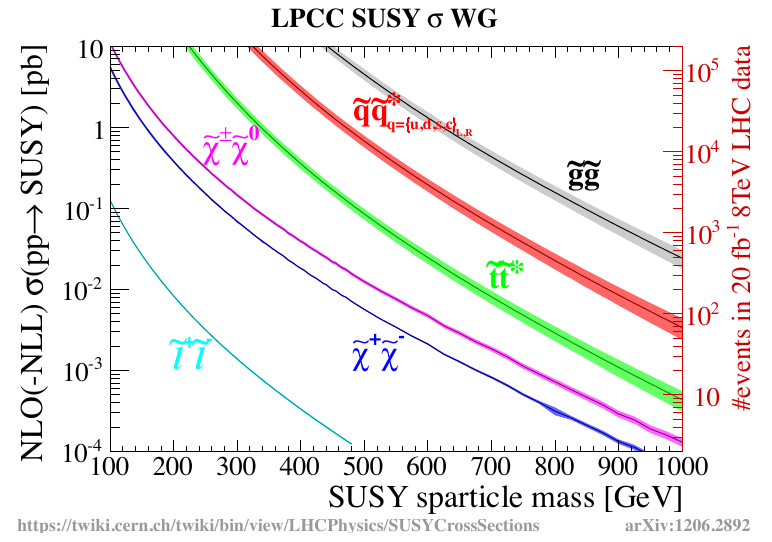
\includegraphics[width=6cm,height=4cm, scale=0.4]{PLOTS/SUSY_Xsec.png}
%\caption{SUSY Production at Hadron Collider}
\end{figure}
\end{varblock}



%\begin{figure}[ht]
%\begin{minipage}[b]{0.45\linewidth}
%\centering
%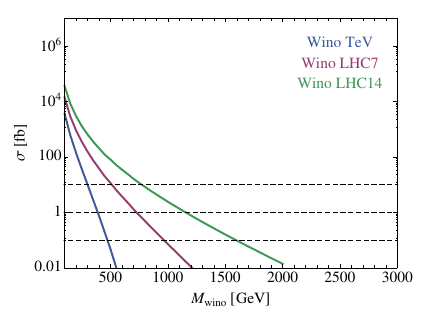
\includegraphics[width=\textwidth]{PLOTS/Weak_SUSY_Production.png}
%\caption{NLO Wino pair production}
%\label{fig:Weak SUSY Production}
%\end{minipage}
%\hspace{0.5cm}
%\begin{minipage}[b]{0.45\linewidth}
%\centering
%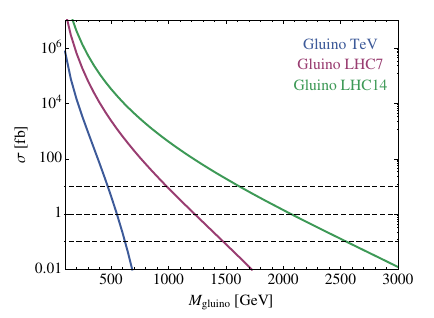
\includegraphics[width=\textwidth]{PLOTS/Gluino_Production.png}
%\caption{NLO gluino pair production}
%\label{fig:Strong SUSY Production}
%\end{minipage}
%\end{figure}


\end{frame}
\section{NLSP Decay}
\begin{frame}
\frametitle{NLSP Decay}
\begin{columns}
\column{0.5\textwidth}
\begin{figure}
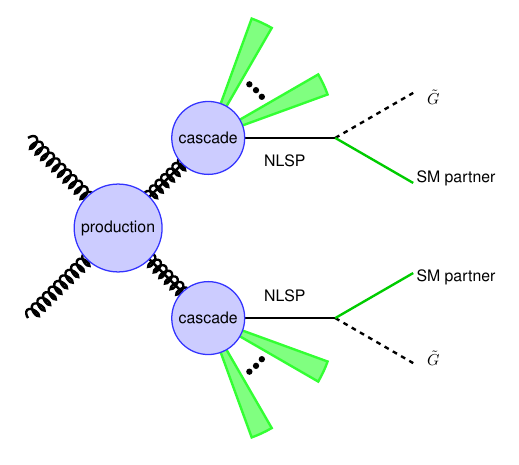
\includegraphics[width=4cm,height=4cm,scale=0.5]{PLOTS/susy-decay.png}
%\caption{Schematic diagram of a GMSB/GGM event}
\end{figure}
\column{0.7\textwidth}
%Cascade Decay of gluino squarks, winos
\begin{table}
\begin{minipage}[b]{1.0\linewidth}\centering
 \begin{tabular}{|l||l|l|}
  \hline
  \multicolumn{3}{|c|}{\bfseries{Cascade Decays}} \\
  \hline 
  \bfseries{Particle} &\bfseries{ Mass }& \bfseries{Decay} \\
   \hline
 $\tilde{g}$ & $M_{\tilde{g}}$ & $\tilde{g}\rightarrow \mbox{j} \tilde{q}^{*}$ \\ 
  \hline
  $\tilde{q}$ & $M_{\tilde{q}}$ & $\tilde{q}\rightarrow \tilde{\chi}^{0}_{1}\mbox{j}, \tilde{g} \mbox{j}$\\
  \hline
   $\tilde{\chi}^{0}_{2}$ & $M_{\mbox{wino}}$ & $\tilde{\chi}^{0}_{2}\rightarrow \tilde{\chi}^{0}_{1}h^{(*)}/Z^{(*)}$\\
  \hline
   $\tilde{\chi}^{\pm}_{1}$ & $M_{\mbox{wino}}$ & $\tilde{\chi}^{\pm}_{1}\rightarrow \tilde{\chi}^{0}_{1}W^{\pm(*)}$\\
  \hline
  \end{tabular}
  \end{minipage}
\end{table}
\end{columns}

\begin{table}
\begin{minipage}[b]{1.0\linewidth}\centering
 %\setlength{\abovecaptionskip}{0pt}
  %\setlength{\belowcaptionskip}{10pt}
 % \topcaption{GMSB,GGM Phenomenology and Relevant final states}
  \begin{tabular}{|l||l||l|}
  \hline
  \multicolumn{3}{|c|}{\bfseries{NLSP Type and Decay Modes}} \\
  \hline 
  \bfseries{NLSP Type} & \bfseries{Decay Mode} & \bfseries{Final states(+ MET )} \\
   \hline
  Bino-Like & $\tilde{\chi}^{0}_{1}\rightarrow \gamma + \tilde{G}$ & $\gamma\gamma,\gamma +\mbox{jets}$ \\ 
  \hline
  Wino-Like & $\tilde{\chi}^{0}_{1}\rightarrow \gamma + \tilde{G}$ & $\ell\gamma,\gamma\gamma,\gamma +\mbox{jets},\ell + \mbox{jets}$\\
  \hline
  Z-rich higgsino & $\tilde{\chi}^{0}_{1}\rightarrow Z/Z^{*} + \tilde{G}$ & $Z(\ell\ell) \mbox{or} Z(\ell^{`}\ell^{`}) + \mbox{jets}$\\
  \hline
  
  \end{tabular}
  \end{minipage}
\end{table}

\end{frame}

\section{NLSP Decay Channels}
\begin{frame}
\frametitle[c]{NLSP Decay Length}
\begin{enumerate}
\item 
The probability for a NLSP produced with energy $\displaystyle{E_{NLSP}}$ in the lab frame to decay before travelling a distance $x$ is given as:
\begin{columns}
\column{0.1\textwidth}
\begin{varblock}[8.7cm]{}
\begin{equation}
\mathcal{P}(x) = 1 - \exp{\left(- \frac{x}{\mathrm{L}} \right)}
\end{equation}
 \end{varblock}
\column{0.5\textwidth}
\begin{varblock}[8.15cm]{}
\begin{equation}
\mathrm{L} = c\tau_{NLSP}\left(\beta\gamma\right)_{NLSP} (mm)
\end{equation}
\end{varblock}
\end{columns}
\item Theory/kinematics
%\begin{columns}
%\column{0.1\textwidth}
\begin{varblock}[16cm]{}
\begin{equation}
c\tau_{NLSP} = 9.9 \times 10^{-8}\frac{1}{k_{1\gamma}}\left(\frac{m_{NLSP}}{100 GeV}\right)^{-5}\left(\frac{\sqrt{\mathrm{F}}}{10TeV}\right)^{4}
\end{equation}
\end{varblock}
%\column{0.5\textwidth}
\begin{varblock}[16cm]{}
\begin{equation}
\left(\beta\gamma\right)_{NLSP} = \frac{|p|}{m_{NLSP}} = \sqrt{\left(\frac{E_{NLSP}}{m_{NLSP}}\right)^{2} - 1}
\end{equation}
\end{varblock}
%\begin{varblock}[6cm]{Decay Lenth}
%$\displaystyle{\feyn{fs f gl f glu f fs}}$

%\begin{fmffile}
%\begin{fmfgraph}(30,3)
%   \fmfset{arrow_len}{cm}\fmfset{arrow_ang}{25}
%   \fmfleft{i}\fmfright{o}\fmf{fermion}{i,o}
%  \end{fmfgraph}
%  \end{fmffile}
%\end{varblock}
%\end{columns}
\end{enumerate}
\end{frame}

\section{NLSP Paramter Space}
\begin{frame}
\frametitle[c]{NLSP Parameter Space}

\begin{enumerate}
\item In GMSB, NLSP decay length is determined by:
    \begin{itemize}
    \item Fundamental SUSY breaking scale is related to the gravitino mass through $\displaystyle{\mathrm{F = m_{3/2}\times\sqrt{3}M_{p}}}$ 
    \item The $m_{NLSP}$ which can be related to $\mathrm{F}$ through $\displaystyle{M_{i} = \frac{\alpha_{i}}{4\pi}N_{5}\Lambda, i = 1, 2, 3 }$
    \item From $\displaystyle{ m_{3/2} =\frac{\mathrm{ \left\langle F \right\rangle}}{\lambda \left\langle F_{S} \right\rangle} \times \frac{\Lambda M_{m}}{\sqrt{3}M_{p}} = C_{grav}\frac{\Lambda M_{m}} {\sqrt{3}M_{p}} } $, 
    Thus, for NLSP to be long-lived $\displaystyle{C_{grav} \gg 1} $ implying $\displaystyle{m_{\tilde{G}} \gg ~eV }$
    \item In MC production, NLSP is long-lived when $C_{grav} \gg 1$ is used and $m_{\tilde{G}} \approx 0 $
        \end{itemize}
\item For GGM, \alert{Is there such a parameter as $C_{grav}$ to change NLSP inherent $c\tau_{NLSP}$}? 
%Would be nice to distinguish it from normal GGM
\item For PGGM, at least the way $c\tau_{NLSP}$ is expressed, the NLSP lifetime depends on model input parameters: $M_{mess}, \Lambda_{G},\Lambda_{S}$
\end{enumerate}
\end{frame}


\section{MC Production}
\begin{frame}
\frametitle{MC Production}
\begin{enumerate}
\item MC production of signal samples for GMSB/GGM/PGGM must span parameter grid space for which:
     \begin{itemize}
      \item NLSP is long lived(reasonable $c\tau_{NLSP}$),
      \item NLSP is boosted,
      \item NLSP is massive enough.
      \item NLSP decays with enough MET.
      \item Consistent with SUSY cross section limits .
     \end{itemize}
\item Tentative Parameter space to scan
\begin{table}
\begin{minipage}[b]{1.0\linewidth}\centering
\begin{tabular}{|l||l||l||l|}
  \hline
  \multicolumn{4}{|c|}{\bfseries{NLSP Parameter Space}} \\
  \hline 
  \bfseries{NLSP Mass} & \bfseries{$c\tau_{NLSP}$} & \bfseries{Parent Mass} & \bfseries{NJets} \\
\hline  
M1,M2 & $C_{grav},\Lambda_{S},\Lambda_{G}$ & M3, $M_{\tilde{q}}$ & $Pt_{jets}$\\
\hline
  \end{tabular}
  \end{minipage}
\end{table}
\item Prelimanary studies using SLHE files from \alert{Yevgeny Kats(GGM)} and \alert{Khoze et al(PGGM)}, however, these SLHE do not allow decay $\tilde{NLSP}\rightarrow \gamma + \tilde{G} $. I used information from GMSB to produce MC samples.
\end{enumerate}

\end{frame}



\section{Sensitivity Study}
\begin{frame}
\frametitle{Sensitivity Study}

\begin{figure}[ht]

\begin{minipage}[b]{0.45\linewidth}
\centering
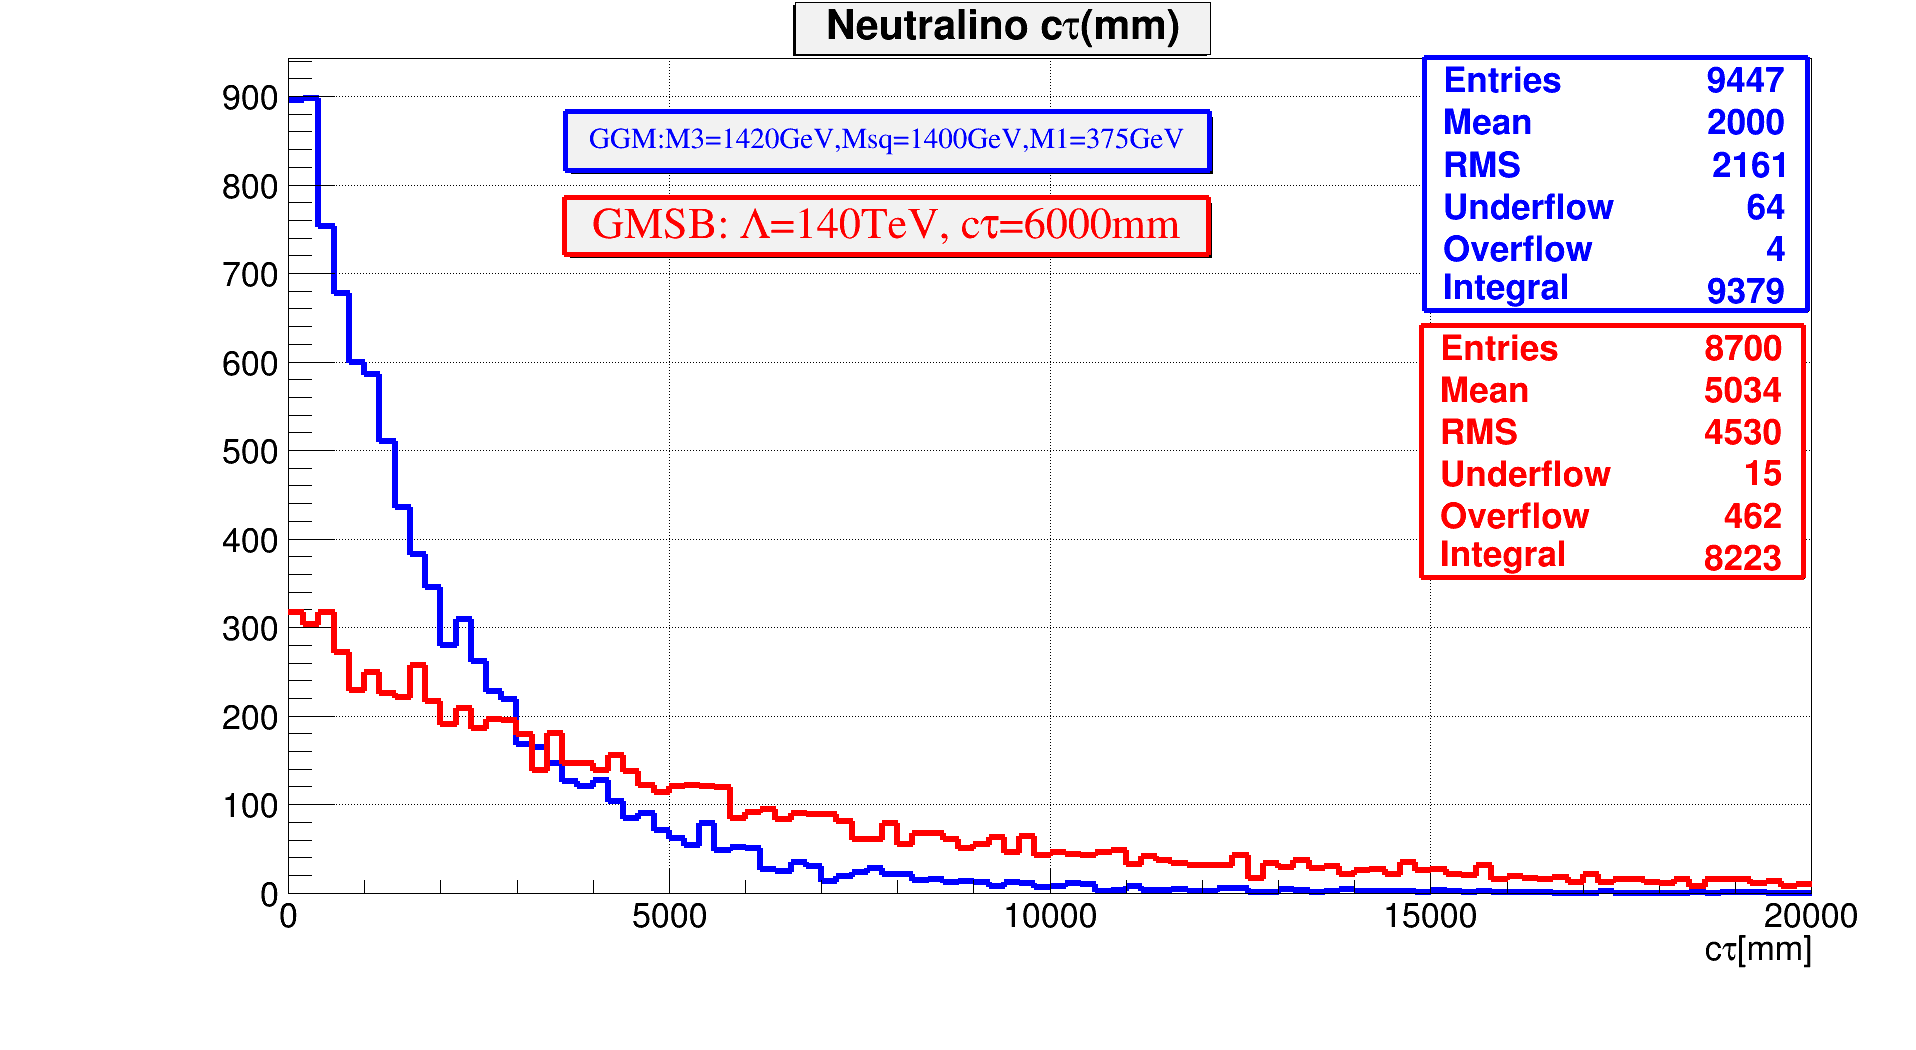
\includegraphics[height=7cm, width=\textwidth]{PLOTS/GMSB_Vs_GGM_Neutralino_ctau.png}
\caption{$c\tau_{\chi^{0}_{1}}$[mm]}
\label{fig:Weak SUSY Production}
\end{minipage}
%\hspace{0.5cm}
\begin{minipage}[b]{0.45\linewidth}
\centering
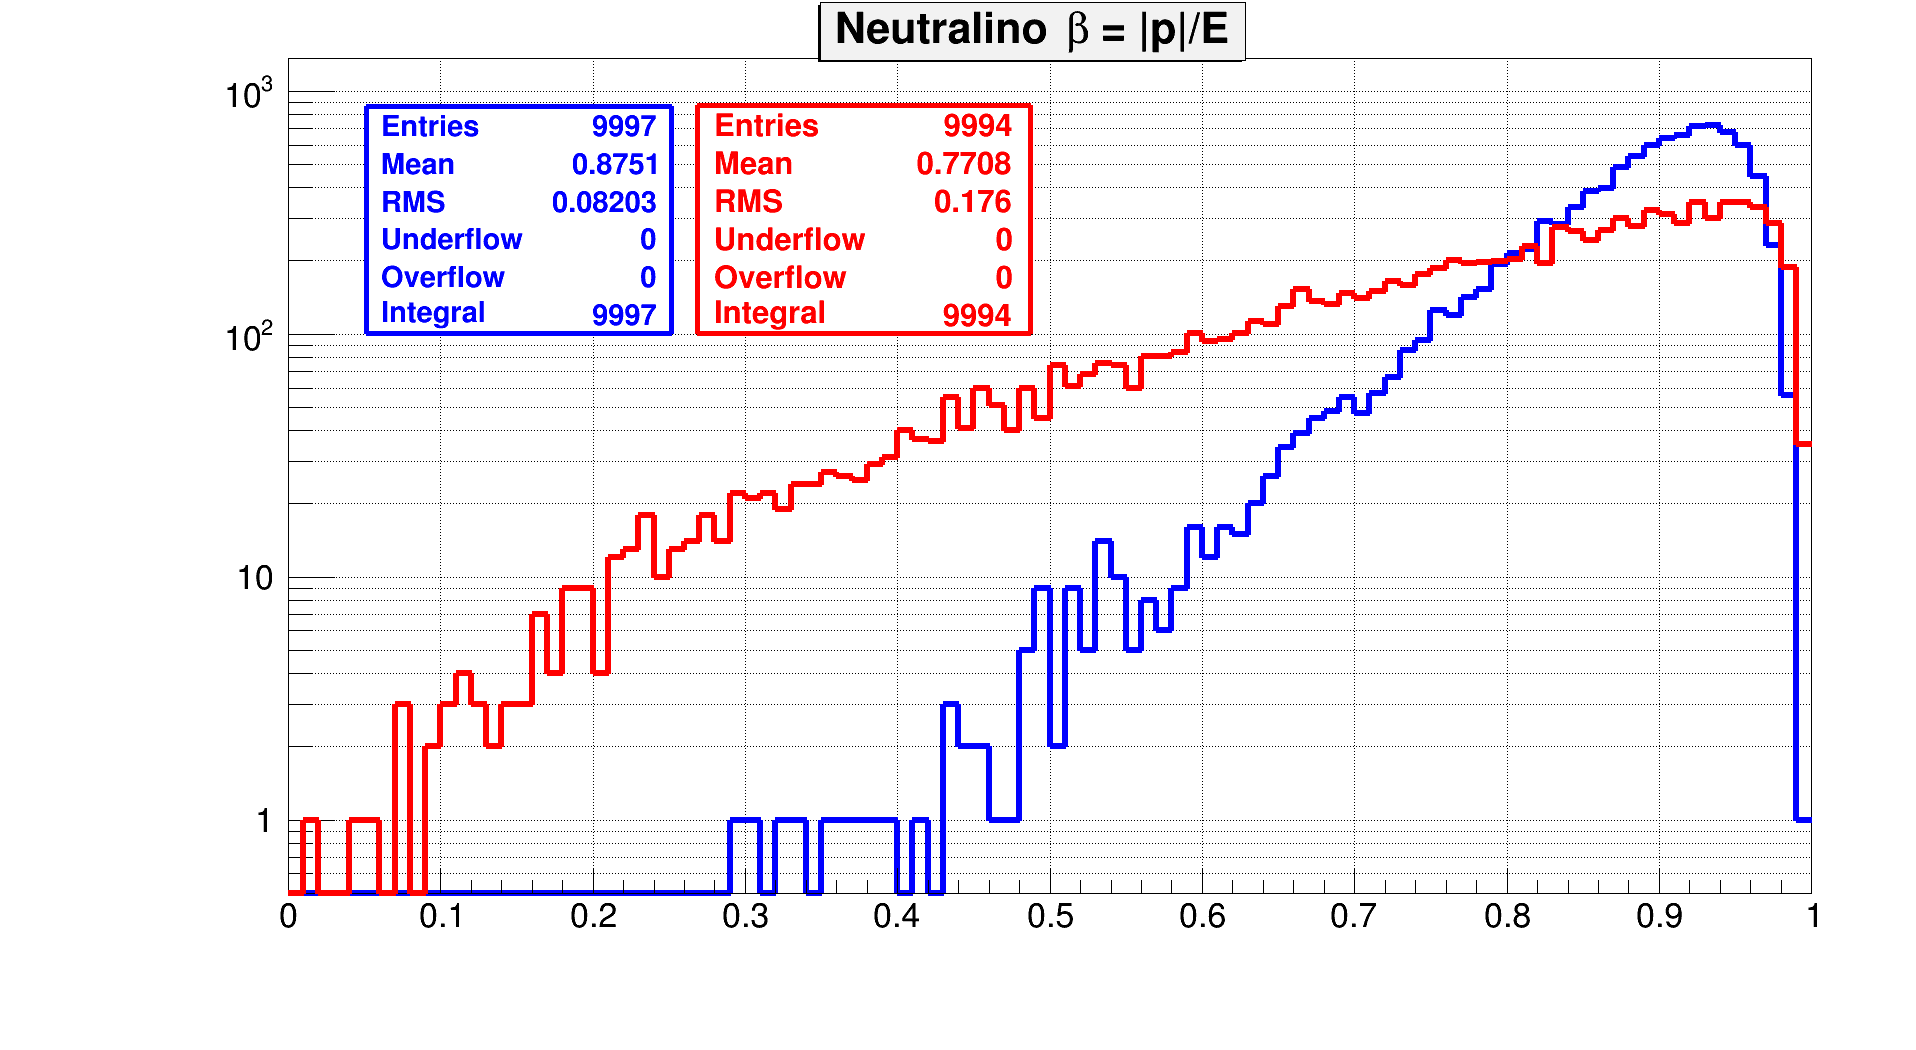
\includegraphics[height=7cm,width=\textwidth]{PLOTS/GMSB_Vs_GGM_Neutralino_Boost.png}
\caption{$Boost_{\chi^{0}_{1}}$ }
\label{fig:Strong SUSY Production}
\end{minipage}
\end{figure}

\end{frame}

%\section*{Text}
%\begin{frame}
%\end{frame}

%\subsection*{Blocks}
%\begin{frame}
%\frametitle{Blocks}
%\begin{definition}[Greetings]
%Hello World
%\end{definition}

%\begin{theorem}[Fermat's Last Theorem]
%$a^n + b^n = c^n, n \leq 2$
%\end{theorem}

%\begin{alertblock}{Uh-oh.}
%By the pricking of my thumbs.
%\end{alertblock}

%\begin{exampleblock}{Uh-oh.}
%Something evil this way comes.
%\end{exampleblock}
%\end{frame}

%%\section{Current Upper Limit}
%%\begin{frame}
%%\frametitle{Delayed Photon + Jet + MET 8TeV}
%%\begin{figure}[ht]
%%\centering
%%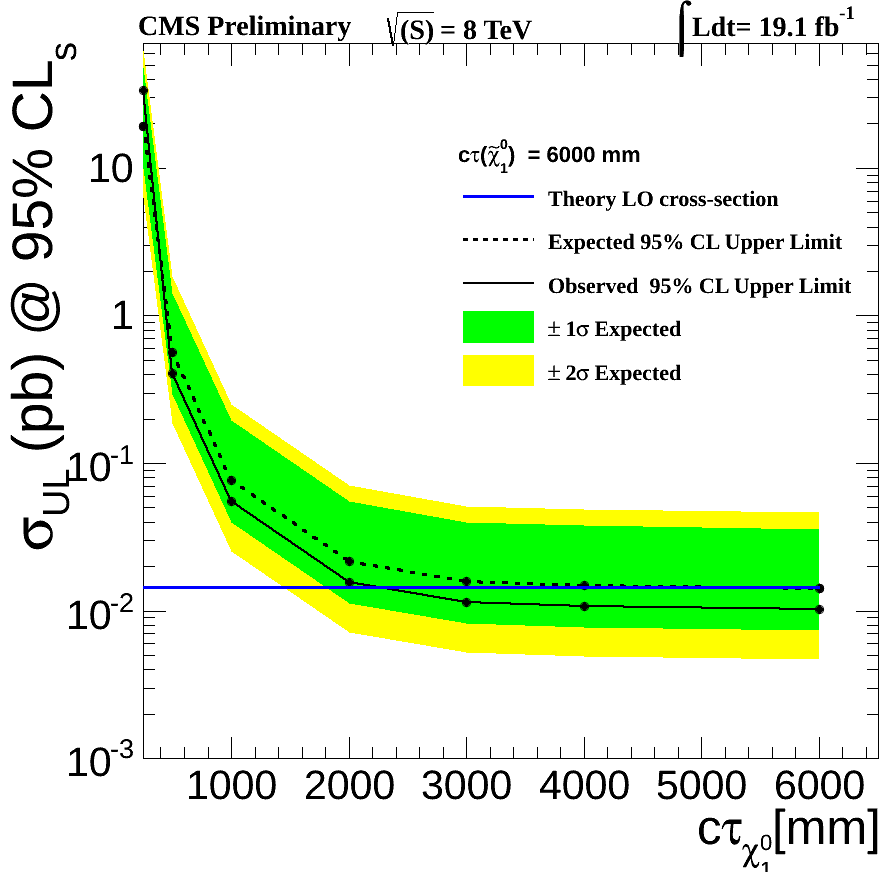
\includegraphics[height=6.5cms,width=\textwidth]{PLOTS/XsecTimesBR_Uplimit_Asymptotic_65Toys.png}
%%\caption{Upper Limit $\chi^{0}_{1}$ Decay}
%%\label{fig:Weak_SUSY UL}

%%\end{figure}
%%\end{frame}

\end{document}